\documentclass[journal,twoside,web]{ieeecolor}
\usepackage{tmi}
\usepackage{cite}
\usepackage{amsmath,amssymb,amsfonts}
\usepackage{algorithmic}
\usepackage{graphicx}
\usepackage{textcomp}
\usepackage{hyperref}
\usepackage[capitalise,noabbrev]{cleveref}
\def\BibTeX{{\rm B\kern-.05em{\sc i\kern-.025em b}\kern-.08em
	T\kern-.1667em\lower.7ex\hbox{E}\kern-.125emX}}
\markboth{\journalname, VOL. XX, NO. XX, XXXX 2024}
{Tan \MakeLowercase{\textit{et al.}}: DeepDWI}


\newcommand{\argmin}{\operatornamewithlimits{argmin}}
\newcommand{\norm}[1]{\left\lVert#1\right\rVert}


\begin{document}
	\title{Diffusion-Weighted Imaging with Learned Nonlinear Latent Space Modeling and Self-Supervised Reconstruction (DeepDWI)}

	\author{Zhengguo Tan, Julius Glaser, Patrick A Liebig, Annika Hofmann, Frederik B Laun, Florian Knoll
		\thanks{This work was supported in part by
			German Research Foundation (DFG)
			under projects 513220538 and 512819079,
			project 500888779 in the Research Unit RU5534
			for MR biosignatures at UHF,
			and by the National Institutes of Health (NIH)
			under grants R01 EB024532 and P41 EB017183.
			In addition, scientific support and HPC resources
			were provided by
			the Erlangen National High Performance Computing Center (NHR)
			of Friedrich-Alexander-University Erlangen-Nuremberg (FAU)
			under the NHR project b143dc.
			NHR is funded by federal and Bavarian state authorities.
			NHR@FAU hardware is partially funded by
			DFG under project 440719683.}
		\thanks{Z.~T. was with the Department
			Artificial Intelligence in Biomedical Engineering (AIBE),
			FAU, Erlangen, Germany.
			He is now with
			the Michigan Institute for Imaging Technology and Translation
			(MIITT),
			Department of Radiology,
			University of Michigan, Ann Arbor, MI 48109 USA
			(e-mail: zgtan@med.umich.edu).}
		\thanks{J.~G. is with the Department Medical Engineering,
			FAU, Erlangen, Germany
			(e-mail: julius.glaser@fau.de).}
		\thanks{P.~A.~L. is with Siemens Healthcare GmbH, Erlangen, Germany
			(e-mail: patrick.liebig@siemens-healthineers.com).}
		\thanks{A.~H. is with the Department AIBE,
			FAU, Erlangen, Germany
			(e-mail: annika.ah.hofmann@fau.de).}
		\thanks{F.~B.~L. is with the Institute of Radiology,
			University Hospital Erlangen,
			FAU, Erlangen, Germany
			(e-mail: Frederik.Laun@uk-erlangen.de).}
		\thanks{F.~K. is with the Department AIBE,
			FAU, Erlangen, Germany
			(e-mail: florian.knoll@fau.de).}
	}

	\maketitle

	% Keep the abstract to 250 words or less.
	\begin{abstract}
		% Define all symbols used in the abstract. Do not cite references in the abstract.
		The code is publicly available at: \url{https://github.com/ZhengguoTan/DeepDWI}.
	\end{abstract}

	\begin{IEEEkeywords}
	Diffusion-weighted imaging, Image reconstruction, Generative AI, Latent space, Self-supervised learning
	\end{IEEEkeywords}

	% ============================== %
	\section{Introduction}
	\label{SEC:INTRO}
	\IEEEPARstart{H}{igh}-dimensional magnetic resonance imaging (HD-MRI)
	has been an emerging and flourishing field,
	which has achieved substantial improvements in terms of spatiotemporal fidelity.
	Instead of the conventional two-dimensional static single-contrast-weighted imaging,
	HD-MRI acquires and reconstructs multi-dimensional information.
	For instance, Brown et al.~\cite{brown_1982_mrsi}
	proposed magnetic resonance spectroscopic imaging (MRSI),
	which uses multiple readout gradients to acquire multiple echo images
	for the computation of spatially resolved metabolic distribution.
	Le BiHan et al.~\cite{lebihan_1986_diff} proposed
	diffusion-weighted imaging (DWI),
	which utilizes spatially and angularly varying
	diffusion encoding gradients in combination with
	fast echo-planar imaging (EPI) readouts \cite{mansfield_1977_epi}
	to obtain multi-contrast diffusion-weighted images
	as a probe into tissue microstructure.
	Ma et al.~\cite{ma_2013_mrf} proposed
	magnetic resonance fingerprinting (MRF)
	which consists of a $T_1$- and $T_2$-prepared pseudo-randomized sequence
	to acquire time-resolved transient-state images
	and a Bloch-equation-based dictionary matching algorithm \cite{doneva_2010_moba}
	for simultaneous quantitative $T_1$ and $T_2$ mapping.

	HD-MRI, however, conventionally requires long scan time.
	Advances in parallel imaging
	\cite{roemer_1990_pi,sodickson_1997_smash,
	pruessmann_1999_sense,pruessmann_2001_gsense,griswold_2002_grappa}
	and compressed sensing
	\cite{lustig_2007_cs,block_2007_cs,liang_2007_psf}
	have enabled accelerated acquisition for HD-MRI.
	In particular, the low-rank modeling and regularization \cite{cai_2010_svt}
	has been a powerful tool in reducing the dimensionality of high-dimensional data,
	which enables accelerated acquisition and high spatiotemporal-resolution reconstruction.
	Usually, singular value decomposition (SVD) is used to
	learn a truncated temporal basis function from
	a large-scale physics-informed dictionary
	\cite{huang_2012_t2basis,lam_2014_spice,mcgivney_2014_svdmrf}.
	The temporal basis function is then integrated
	with the MRI forward model,
	i.e.~the sensitivity encoding operator \cite{pruessmann_2001_gsense},
	for joint reconstruction of the corresponding spatial basis images.
	In addition, low-rank regularization can be employed in the joint reconstruction
	\cite{tamir_2017_t2shuffling}.

	Beyond the low-rank technique,
	advanced neural networks, e.g.~autoencoder \cite{hinton_2006_ae},
	have been explored for HD-MRI reconstruction and
	proven to supply more accurate representations of high-dimensional data than SVD.
	Lam et al.~\cite{lam_2019_mrsi} and Mani et al.~\cite{mani_2021_qmodel} proposed
	to first learn a denoising autoencoder (DAE) model
	from a physics-informed simulated dictionary
	and then incorporate the learned DAE model as a regularizer
	in iterative reconstruction.
	Further, Arefeen et al.~\cite{arefeen_2023_latent} proposed
	to replace the conventional SVD-based linear subspace modeling
	\cite{huang_2012_t2basis}
	by the latent decoder model within DAE
	for improved $T_2$-weighted image reconstruction.
	The capability of DAE to learn diffusion MRI models, however,
	is open to questions.
	DAE is composed of sequential fully connected layers
	with nonlinear activation functions.
	This simple architecture may fail to learn complicated functions.
	DWI signal is such an example.
	The standard diffusion tensor model \cite{basser_1994_dmri}
	consists of six tensor elements,
	and forms DWI signals based on the multiplication of exponential functions.
	Moreover, DWI signals can be described with more complicated models,
	e.g.~the ball-and-stick model \cite{behrens_2003_ballstick},
	which involves even more parameters.

	Besides learning a \textit{prior} based on simulated data
	for regularization or latent space modeling,
	Hammernik et al.~\cite{hammernik_2018_varnet} and
	Aggarwal et al.~\cite{aggarwal_2018_modl}
	proposed supervised learning unroll reconstruction networks,
	which are trained by fully sampled in vivo data.
	Yaman et al.~\cite{yaman_2020_ssdu,yaman_2022_zs}
	proposed the self-supervised learning unroll network
	without fully-sampled data,
	which builds upon the concept of cross-validation in machine learning.
	However, in the case of DWI,
	it is rather challenging to acquire fully-sampled data
	for the training of a regularization functional.
	First, fully-sampled DWI requires a longer echo train in EPI,
	which not only elongates the scan time
	but also increases off-resonance-induced geometric distortion.
	Second, there exists a wide range of diffusion acquisition modes,
	thereby requiring a larger dataset than the two-dimensional imaging scenario.

	In this work, we aim to develop a generalized DWI reconstruction framework
	with learned nonlinear latent space modeling and self-supervised reconstruction,
	dubbed DeepDWI.


	% ============================== %
	\section{Related Work}

    \begin{figure*}
		\centering
		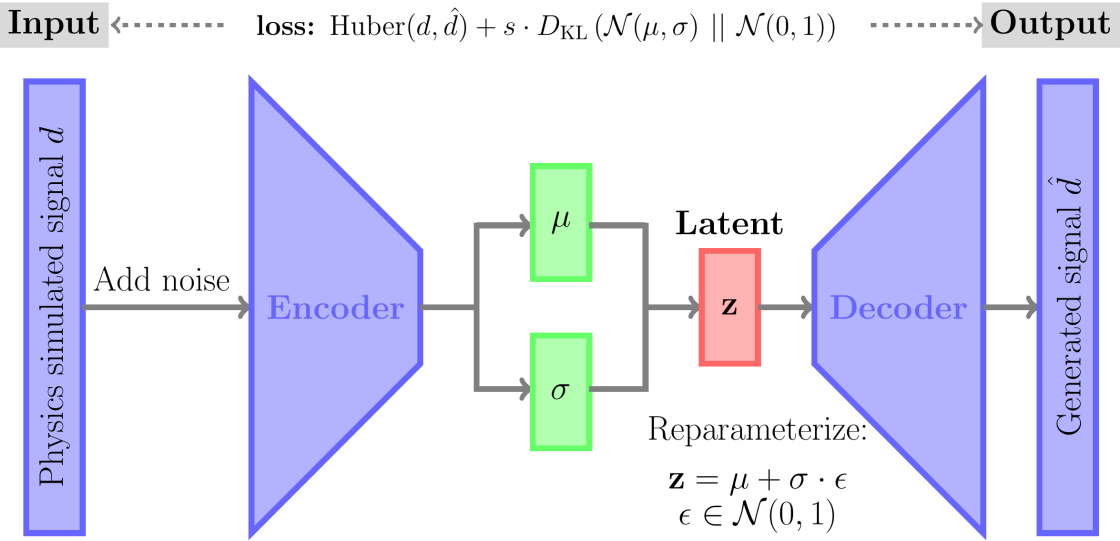
\includegraphics[width=\textwidth]{../figures/fig1.png}
		\caption{\textbf{(A)} The architecture of a variational autoencoder.
            \textbf{(B)} An illustration of the joint $k$-$q$-slice forward operator
            for multi-band multi-shot DWI acquisition.
            $[x, y, z, q]$ denotes the shape of input DWI ($\mathbf{\tilde{x}}$),
            with $x$ and $y$ as the image size, $z$ as the number of slices,
            and $q$ as the number of diffusion encodings.
            The operator outputs multi-dimensional $k$-space with the shape $[x, y, 1, c, q, s]$,
            with $c$ as the number of receiver coils, $s$ as the number of shots.}
		\label{FIG:MODEL}
	\end{figure*}

    \subsection{Variational Autoencoder (VAE)}

    \cref{FIG:MODEL} (A) illustrates the VAE model.
    Pioneered by Kingma and Welling \cite{kingma_2014_vae},
    VAE is a deep generative model,
    which learns the true distribution of input training data $x$.
    To achieve this, VAE

    \subsection{Multi-Band Multi-Shot DWI Acquisition \& Modeling}

    \cref{FIG:MODEL} (B) illustrates the joint $k$-$q$-slice forward forward operator
    for multi-band multi-shot DWI acquisition \cite{tan_2024_naviepi}.
    This operator can be understood as
    an extended sensitivity encoding (SENSE) operator \cite{pruessmann_2001_gsense},
    which maps the multi-slice multi-diffusion-weighted images ($\mathbf{\tilde{x}}$)
    to their corresponding $k$-space,
    \begin{equation}
        \mathcal{A}(\mathbf{\tilde{x}}) = \mathbf{P \Sigma \Theta F S \Phi} \mathbf{\tilde{x}}
        \label{EQU:FWD}
    \end{equation}
    Here, the images $\mathbf{\tilde{x}}$ are point-wise multiplied
    with the pre-computed shot-to-shot phase variation maps ($\mathbf{\Phi}$)
    and coil sensitivity maps ($\mathbf{S}$).
    The output images are then converted to $k$-space
    via two-dimensional fast Fourier transform ($\mathbf{F}$),
    point-wise multiplied with the multi-band phases ($\mathbf{\Theta}$),
    summed along the slice dimension ($\mathbf{\Sigma}$),
    and then multiplied by the undersampling mask ($\mathbf{P}$).

    With the operator $\mathcal{A}$, the inverse problem in DWI reads,
    \begin{equation}
        \argmin_{\mathbf{\tilde{x}}} \norm{\mathbf{y} - \mathcal{A}(\mathbf{\tilde{x}})}_2^2 + \lambda \mathcal{R}(\mathbf{\tilde{x}})
        \label{EQU:INV}
    \end{equation}
    where $\mathbf{y}$ is the measured $k$-space data,
    and $\mathcal{R}(\hat{x})$ is the the regularization function
    with the regularization strength $\lambda$.
    When using the Tikhonov regularization,
    i.e.~$\mathcal{R}(\mathbf{\tilde{x}}) = \norm{\mathbf{\tilde{x}}}_2^2$,
    \cref{EQU:INV} can be solved via the conjugate gradient (CG) method.
    When using non-smooth regularization functions,
    e.g.~locally low rank (LLR) as in our previous work \cite{tan_2024_naviepi},
    $\mathcal{R}(\mathbf{\tilde{x}}) = \norm{T(\mathbf{\tilde{x}})}_*$,
    where singular value thresholding \cite{cai_2010_svt} is computed
    to enforce low rankness in the spatial-diffusion matrices $T(\mathbf{\tilde{x}})$,
    the alternating direction method of multipliers (ADMM) \cite{boyd_2010_admm}
    is used to solve \cref{EQU:INV}.


    \subsection{Zero-Shot Self-Supervised Learning (ZSSSL)}


	% ============================== %
	\section{Methods}



	% ============================== %
	\section{Results}

	\subsection{VAE enables robust \& accurate learning of DWI signal}

	\subsection{Zero-shot learning enables motion-robust DWI}

	\subsection{Zero-shot learning: model generalization}

	\subsection{VAE modeling with zero-shot learning reconstruction}


	% ============================== %
	\section{Discussion}


	% ============================== %
	\section{Conclusion}


	% ============================== %
	\section*{Acknowledgment}

	Z.~T. thanks to Ms.~Soundarya Soundarresan for
	her work and discussion on denoising autoencoder.
	Z.~T. thanks to Dr.~Xiaoqing Wang for
	the discussion on self-supervised learning.

	% ============================== %
	\bibliographystyle{IEEEtran}
	\bibliography{../../ref/ref}

\end{document}
